\section{Network of \emph{parameterization prediction}}
In this section, we first explain the general structure of our proposed network, and then in Sec~\ref{subsec:k-n_point_net} and Sec~\ref{subsec:semnet} we explain the details of its structure.
\subsection{Network overview}
\begin{figure}[htbp]
	\centering
	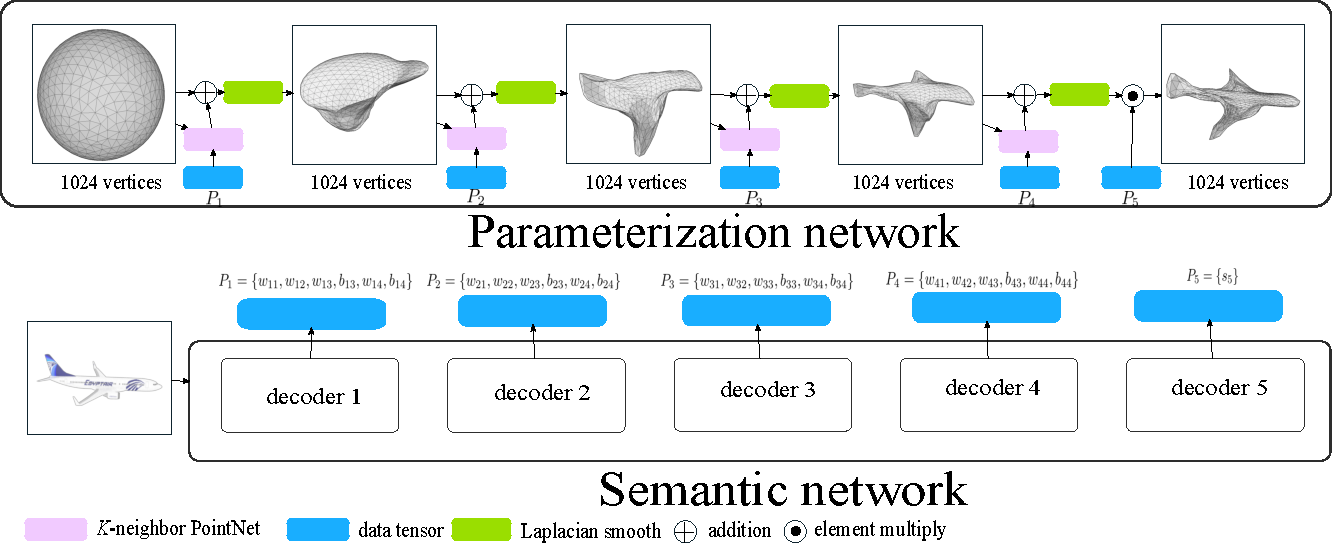
\includegraphics[width=\linewidth]{img/net/overview}
	\caption{The overview of the network: The proposed network consists of two sub-networks. One is the parameterization network that maps points sampled from a unit sphere surface to target shape. The other is the semantic network that takes image as input and predict parameters for the parameterization network. In the figure two version of implementation of parameterization network is shown. Comparing to $\alpha$ version, the $\beta$ version starts with fewer point samples and the point number is increased by mesh-based upsampling in the following layers}
	\label{fig:overview}
\end{figure}
Our basic idea is to use convolution and deconvolution network that takes image as input to predict parameters for the parameterization network that deform/map a point set uniformly sampled from the surface of a unit sphere to the target shape. Figure~\ref{fig:overview} illustrates the overview of our network. The parameterization network is built by stacking several K-neighbor PointNet (explained in Sec~\ref{subsec:k-n_point_net}). Each k-neighbor point net predicts a point-wise offsets and add them to the sampled points. In this way, the parameterization network can map a randomly sampled point set to target shape. By using different randomly generated samples from the parameter domain in the training and testing, the parameterization network can simulate the \textit{sampling variation} that is introduced by using specific point set as ground truth. The semantic network is built by convolution and deconvolution layers, it takes image as input to predict the parameter for the parameterization network. In this way, the semantic network relates the input image to the shape manipulation. The entire network is built by differentiable operations, making it end-to-end trainable.
\subsection{ \textit{K}-neighbor PointNet for parameterization network} 
\label{subsec:k-n_point_net}
\begin{figure}[htbp]
	\centering
	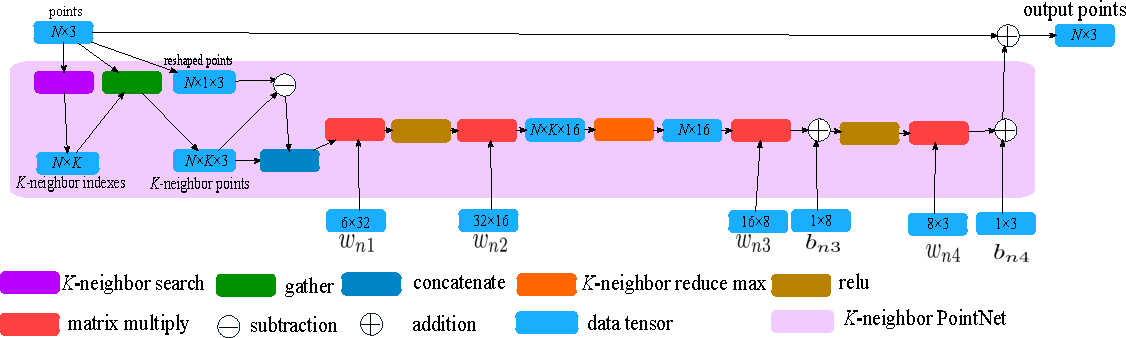
\includegraphics[width=\linewidth]{img/net/k-n_pointnet}
	\caption{The structure of \textit{K}-neighbor PointNet: }
	\label{fig:knpointnet}
\end{figure}
An essential building block for our parameterization network is K-neighbor PointNet. Figure~\ref{fig:knpointnet} shows the internal structure of K-neighbor PointNet. The proposed structure is inspired by and named after PointNet\citep{PointNet} and its follow-up PointNet++\citep{NIPS2017_7095}. K-neighbor PointNet is a network forged with the symmetric functions and apply it on each k-neighbor of input point set to predict a drift for the center of these k-neighborhoods. We propose such structure for two reasons. Firstly, we tried to forge the parameterization network as multi-layer perception network and failed to train it to output any meaningful result. Secondly, we propose such structure after consider human activity. When a potter crafting something from a lump of clay, she do it by applying a serious of squeeze. Each squeeze only affect the clay locally, but all the squeeze together turn the clay into graceful shape. Our parameterization network is designed to simulating such serial local process. 
\subsection{Mesh Based Upsampling}
The building block used in the $\beta$ version of the parameterization network.
\subsection{Semantic network}
\label{subsec:semnet}
\begin{figure}[htbp]
	\centering
	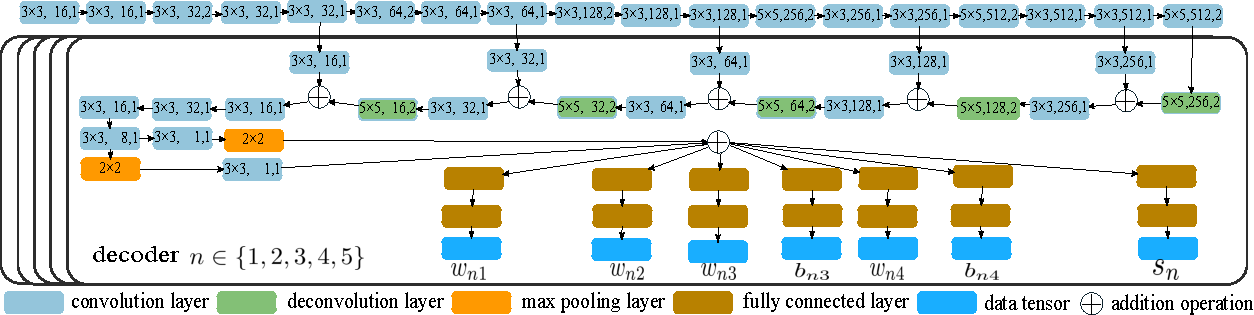
\includegraphics[width=\linewidth]{img/net/semnet}
	\caption{Semantic network: The semantic network takes image as input and predict parameters for the \textit{K}-neighbor PointNet and the global scale operation in the parameterization network. The semantic network have separate decoders for each \textit{K}-neighbor PointNet and and the global scale operation.}
	\label{fig:conv}
\end{figure}
In our semantic network, we use convolution layers to extract semantic features from input image. In order to encode the \textit{semantic variation}, a random feature mapped from the normal distributed random vector is concatenated to the semantic feature.  Figure~\ref{fig:conv} shows the detailed structure for this part. 
\subsection{Losses}
\noindent{\textbf{Chamfer Loss}} The Chamfer distance is directly borrowed from \citep{PSGN}. This loss can drive the output point set to approach the target, but it is not sufficient for a smooth and  
\begin{equation}
l_c = \sum_x \min||x-y||_2^2+\sum_y \min||x-y||_2^2
\end{equation}

\noindent{\textbf{Regularization}}
Edge variation regularization 
idealy if the surface is covered with 

